\paragraph{Scale-Location Plots, Testing Whether $\mathrm{Var}(\varepsilon) = const$}
	These plots plot the absolute values of the standardized residuals versus the predicted values. 
	
	\begin{enumerate}
	  	\item A single smoothing curve is being fitted to the plotted data (displayed in red below).  
	  		\begin{itemize}
	  		  \item This curve displays the behaviour of the standard residuals based on the complete data.
	  		  \item This curve should ideally be constant.
	  		\end{itemize}
	  	\item More smoothing curves are fitted to the plotted data. 
	  		\begin{itemize}
	  		  \item For these curves samples are taken out of the data, from which the standard residuals are calculated and plotted to the data (displayed in light grey below).
	  		  \item If the residual plot of the complete data is not close to constant, these sample residual plots can be analyzed in order to find out whether this behaviour is due to a random effect.
	  		\end{itemize}
	  	\end{enumerate}	
	
	\textbf{The model fits the data well} if the smoothed residual line is close to constant, if it is not, then one can assume that it is due to a random effect, if the red line from the example below is within the grey band, in which case there seems to be constant variance.
	
	\RCode
	{
		Creating a Scale-Location Plot
	}
	{
		sections/RegressionAnalysis/ResidualAnalysis/DiagnosticsInstruments/ScaleLocation/Code.R
	}
	
	\begin{figure}[H]\centering
		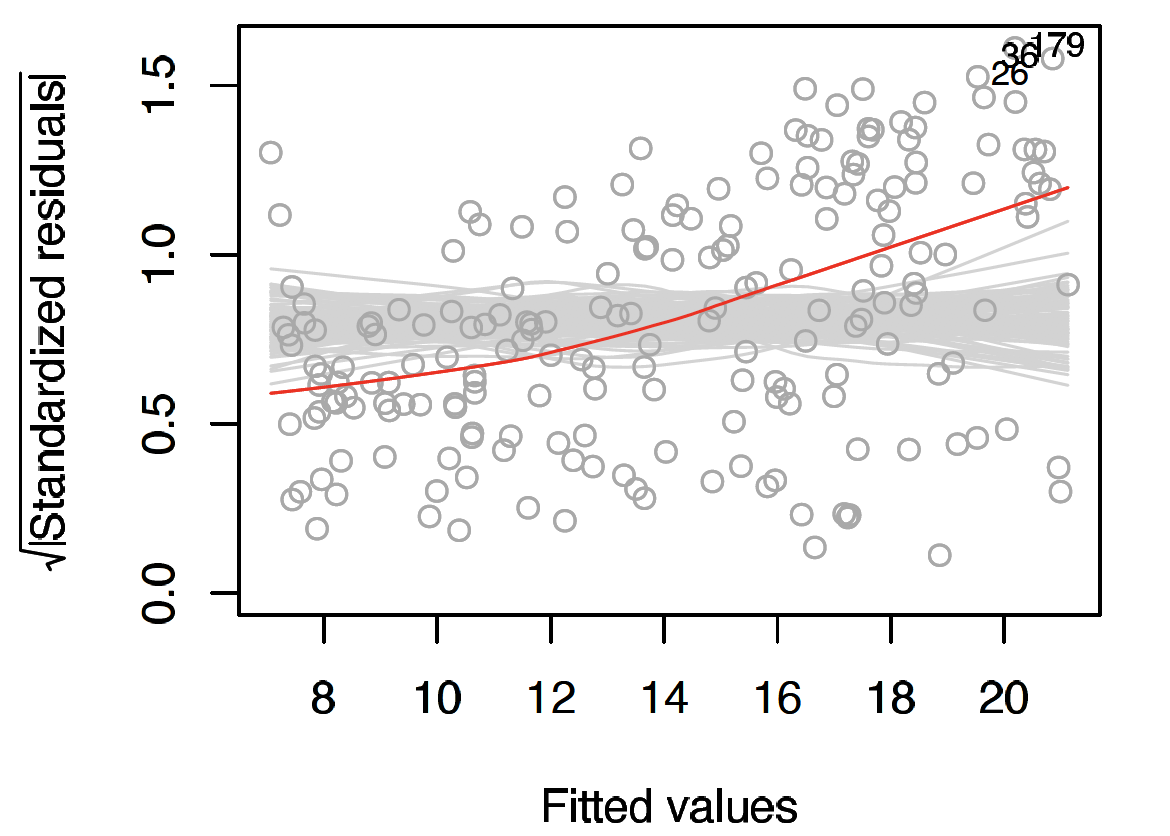
\includegraphics[width=0.6\linewidth]{images/ScaleLocation.png}
		\caption{Scale location plot with smoothing curve (in red) and simulated smoothing curves fitted on the basis of resampled data (in grey).}
	\end{figure}